% \documentclass[letterpaper, 12 pt, conference]{ieeeconf}  % Comment this line out
                                                          % if you need a4paper
\documentclass[a4paper, 10pt, conference]{ieeeconf}      % Use this line for a4
                                                          % paper

\IEEEoverridecommandlockouts                              % This command is only
                                                          % needed if you want to
                                                          % use the \thanks command
\overrideIEEEmargins
% See the \addtolength command later in the file to balance the column lengths
% on the last page of the document



% The following packages can be found on http:\\www.ctan.org
\usepackage{graphicx} % for pdf, bitmapped graphics files
\usepackage{bm}
\usepackage{lipsum}
\newcommand{\uvec}[1]{\boldsymbol{\hat{\textbf{#1}}}}
%\usepackage{epsfig} % for postscript graphics files
%\usepackage{mathptmx} % assumes new font selection scheme installed
%\usepackage{times} % assumes new font selection scheme installed
%\usepackage{amsmath} % assumes amsmath package installed
%\usepackage{amssymb}  % assumes amsmath package installed

\title{\LARGE \bf
\LaTeX~Paper
}

\author{Author1$^{1}$ and Author2$^{2}$% <-this % stops a space
\thanks{}% <-this % stops a space
\thanks{$^{1}$Author1, 13116053, Department of Electronics and Communication Engineering}%
\thanks{$^{2}$Author2, 13116054, Department of Electronics and Communication Engineering}%
}


\begin{document}



\maketitle
\thispagestyle{empty}
\pagestyle{empty}


%%%%%%%%%%%%%%%%%%%%%%%%%%%%%%%%%%%%%%%%%%%%%%%%%%%%%%%%%%%%%%%%%%%%%%%%%%%%%%%%
\begin{abstract}

 \lipsum[1-2]



\end{abstract}


%%%%%%%%%%%%%%%%%%%%%%%%%%%%%%%%%%%%%%%%%%%%%%%%%%%%%%%%%%%%%%%%%%%%%%%%%%%%%%%%
\section{FIRST SECTION}

\lipsum[1-3]

\section{SECOND SECTION}
\lipsum[1]


\subsection{Sub Section1}

\lipsum[1-3]
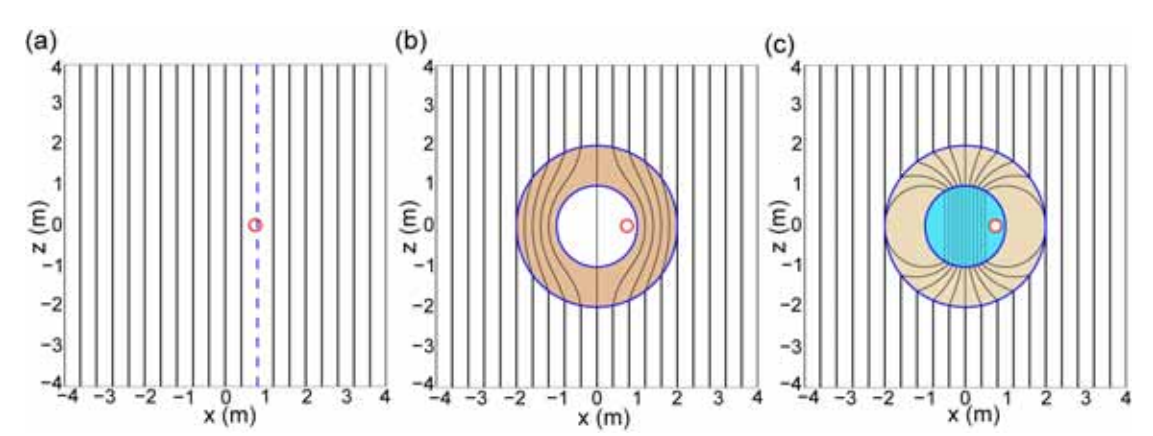
\includegraphics[scale=0.25]{1}

\subsection{Sub Section2}

\lipsum[1]



\subsection{Sub Section3}
\lipsum[1-2]

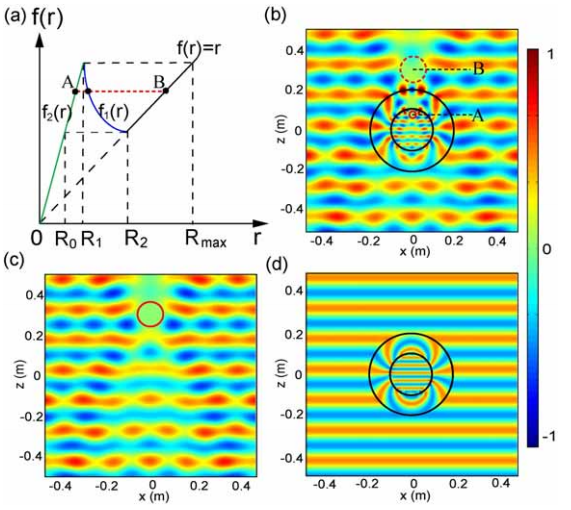
\includegraphics[scale=0.55]{2}

     

\begin{thebibliography}{99}

\bibitem{c1} 1.	 Yan, M.; Ruan, Z.; Qiu, M. (2007). "Cylindrical Invisibility Cloak with Simplified Material Parameters is Inherently Visible".
\bibitem{c2} Ruan, Z.; Yan, M.; Neff, C. W.; Qiu, M. (2007). "Ideal Cylindrical Cloak: Perfect but Sensitive to Tiny Perturbations". 
\bibitem{c3}Greenleaf, A.; Kurylev, Y.; Lassas, M.; Uhlmann, G. (2007). "Improvement of cylindrical cloaking with the SHS lining".
\bibitem{c4} Yu Luo, Jingjing Zhang, Hongsheng Chen, Bae-Ian Wu, and Jin Au Kong(2007). "A new strategy to conceal an object from electromagnetic wave"





\end{thebibliography}




\end{document}
